\documentclass[10pt,letterpaper,final]{report}
\usepackage[margin=1in]{geometry}
\usepackage[utf8]{inputenc}
\usepackage{amsmath}
\usepackage{amsfonts}
\usepackage{amssymb}
\usepackage{amsthm}
\renewcommand\qedsymbol{$\blacksquare$}
\usepackage{enumerate}
\usepackage{hyperref}
\usepackage{pdfpages}
\usepackage{graphics}
\usepackage{graphicx}
\usepackage{tikz}
\usepackage{tikz-qtree}
\usetikzlibrary{automata,arrows}
\usepackage{mdframed}
\usepackage[
  backend=biber,
  style=numeric-comp,
  sorting=none
]{biblatex}
\addbibresource{references.bib}

\usepackage{minted}
\usemintedstyle{algol_nu}
\usepackage{xltabular}
\usepackage{pdflscape}
\usepackage{multicol}
\usepackage{underscore}
\usepackage{changepage}

\NewDocumentCommand{\sourcefile}{m v}{
  \subsection{\texttt{#2}}\label{sec:#2}
  \inputminted[linenos,breaklines,breakanywhere=true,fontsize={\fontsize{6pt}{7pt}\selectfont}]{#1}{#2}
}

% Based on template from COSC-417 at Towson University, originally authored by Marius Zimand

\renewcommand{\thesection}{\arabic{section}}

\begin{document}
\begin{center}
  \fbox{
    \vbox{
      \begin{flushleft}
        Jonathan Llovet \\  % authors' names
        EN.605.202.81 \\  %class
        2026-06-23 \\  % date
        Lab 1 \\ % ID
      \end{flushleft}
      \center{\Large{\textbf{Recursion - Converting Prefix to Postfix Expressions}}}
      %\end{mdframed}
    } % end vbox
  } % end fbox
  \vline
\end{center}

\noindent\textbf{Prompt:}

In this assignment you will use recursion to convert prefix expressions directly to postfix expressions. You may not use a stack as you did in Lab 1.

Write a program that accepts a prefix expression containing single letter operands and the operators \texttt{+, -, *, /,} and \texttt{\$} (representing exponentiation). Output the corresponding postfix expression.  For example, if your input is \texttt{*AB} then output should be \texttt{AB*}. Output of \texttt{BA*} is considered incorrect. In your analysis, be sure to discuss why recursion makes sense. Consider your recursive solution with your iterative solution from Lab 1. Is one better than the other? Do you feel differently than you did when you wrote Lab 1. Tell us what you learned and what you would do differently. Be sure to review the Programming Assignment Guidelines for specific requirements for the Analysis and before submitting this assignment.

Don't forget to do reasonable error checking and try to make your error messages specific and helpful. You may not use library functions. You must write your own code. You must read and write from named files.

\noindent \textbf{Additional guidelines from instructor:}

\begin{itemize}
  \item Whitespace should be quietly stripped out (skipped) on a per character basis.
  \item You should not accept characters outside of the bounds of what you accept. If you choose to only accept the valid operator characters \$*/+- and alphabetical characters that is fine. There is no reason to accept any other characters. I recommend using your language's version of \texttt{isAlpha()} to determine if a non operator character is valid.
  \item Numeric literals are up to you, however, I would recommend not accepting (and raising errors) for integer literals. Namely, it is a very hard problem to handle:
  \begin{itemize}
    \item Consider \texttt{+123}. Is it \texttt{1 + 23}, \texttt{12 + 3}, or \texttt{123 +} a missing a value? If you decide to use numeric literals, you must detail in your readme and analysis, providing the rules required for numeric integers, how they can be formed, and of course have matching code to enforce those rules.
    \item Even if you don't use numeric literals, your readme should clearly state what character sets are acceptable.
  \end{itemize}
\end{itemize}

\tableofcontents

\pagebreak

\section{The Problem to Solve}

This lab illustrates the use of recursion in the conversion of prefix expressions to postfix expressions. The prefix expressions will be read in from a file and then output to a file, both of which are provided at the command line. Errors will be printed to stderr for review. The lab is meant to be run as a module. See \texttt{README.md} for running instructions.
We want to convert expressions in this form: \texttt{+AB} to this form \texttt{AB+}. Both of these are equivalent to the probably more familiar infix notation for the same expression \texttt{A+B}. Put another way, we want to convert from Polish notation to Reverse Polish notation \parencite{EnWikipediaorgReversePolishNotation}.

The program should satisfy the following:

\begin{enumerate}
  \item Transform a prefix (Polish) expression to an equivalent postfix (Reverse Polish) expression
  \item Use a recursive (as opposed to an iterative) implementation of the algorithm for doing so
  \item Handle expressions with single-letter alphabetic operands and the operations \verb|+, -, *, /, $|
  \item Be callable from the command line as a Python module
  \item Read an input file specified at the command line
  \item Output results to an output file specified at the command line
  \item Output errors related to invalid input to the user
  \item Report issues in a helpful way to the user
  \item Have reasonable error handling
  \item Produce no other side effects other than writing logs
\end{enumerate}

\section{Strategy}\label{sec:strategy}

Since lab2 is a variation on lab1, there were many components of lab1 that I was able to reuse for lab2. Some things of note: there were refinements to my understanding of the problem specification that were previously enforced by tets, and in the course of lab2, I had to not only update the implementation of the solution but also change requirements imposed by my tests on my code. As I discuss in \ref{sec:testing}, I do not think that my handling of this was as elegant as it should have been, but regardless the use of test-driven development ultimately is what enabled me to produce a working solution and to excise a large amount of code that is no longer needed.

Also notable about lab2 is that I have predominantly replaced the stack-based approach of lab1 with a tree-based approach in lab2. Why a tree? The tree is a naturally recursive data type, which lends itself well to the recursive character of the problem we are faced with. Additionally, prefix, infix, and postfix expressions all share a core structure that is embodied in an abstract syntax tree (AST), which is a structure frequently used in parsers. My strategy overall was to convert the prefix expression into an AST, then to simply read off the postfix expression from the AST by reading the nodes in post-order. At the suggestion of my professor, I constrained the core portion of the conversion to a single pass over the input expression. This constraint, along with the requirement to have this be a recursive solution, made the generation of the AST the trickiest part of the program. As the input expression is read, I check for error states based on the partial information available at that point in the reading of the expression. In some cases, this means that the program can reject the input expression in sometimes significantly less than linear time, but the runtime overall is $O(n)$.

What follows is a description of the core flow of the program. First, the IO portion from the command line and the main portion that drives the program.
\begin{figure}[ht]
  \centering
  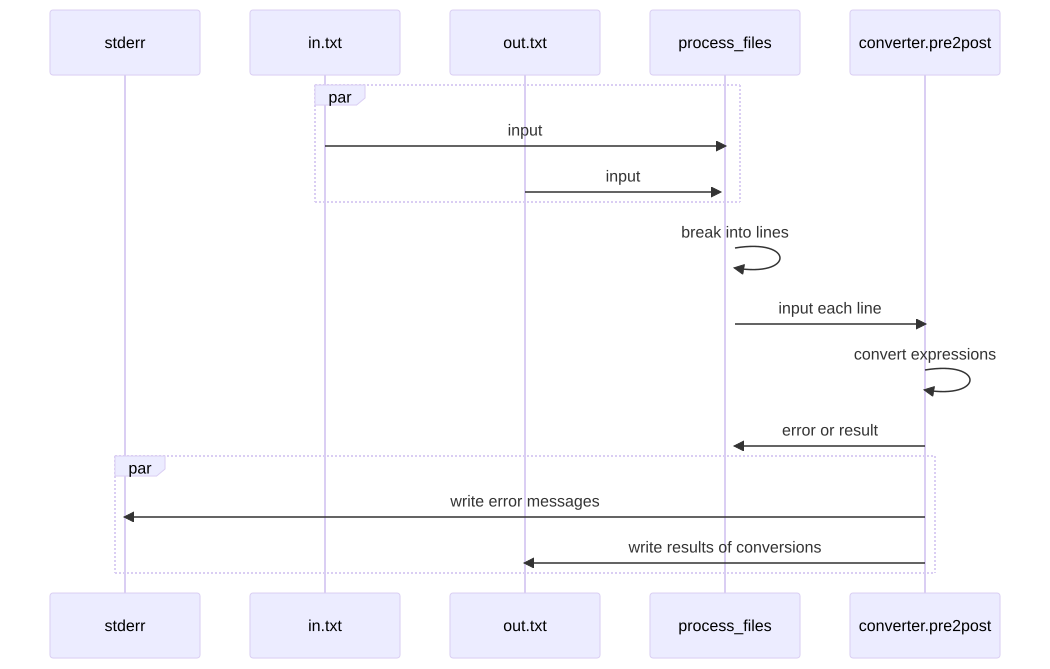
\includegraphics[width=0.9\linewidth]{lab2-strategy-io.pdf}
  \caption{Core IO flow}\label{fig:strategy-io}
\end{figure}

The IO flow above calls into the conversion flow, which is sketched below.

\begin{figure}[ht]
  \centering
  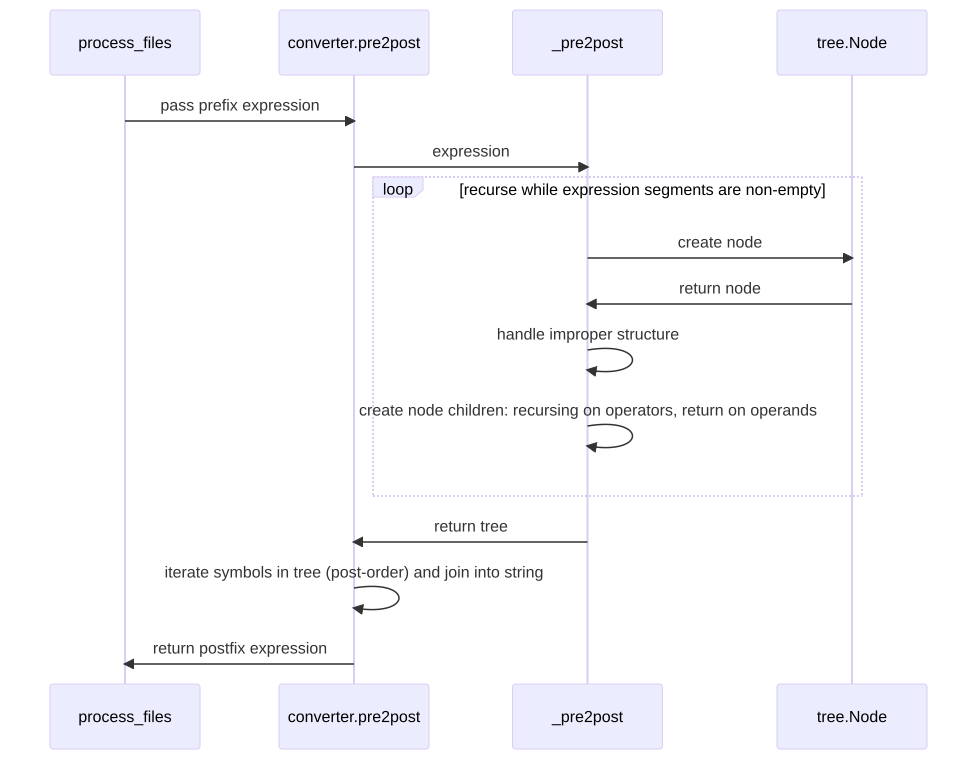
\includegraphics[width=0.9\linewidth]{lab2-strategy-conversion.pdf}
  \caption{Conversion flow}\label{fig:strategy-conversion}
\end{figure}

The validation flow is the next layer down. It is sketched below. Details about conditions that are checked can be seen in \texttt{lab2/convert/converter.py} and \texttt{lab2/parse/validate.py}.

I removed the evaluation flow in lab2 in order to simplify the project. The interpreter that I built in lab1 was valuable in some ways, but it did not add enough to warrant re-implementing recursively.

\begin{figure}[ht]
  \centering
  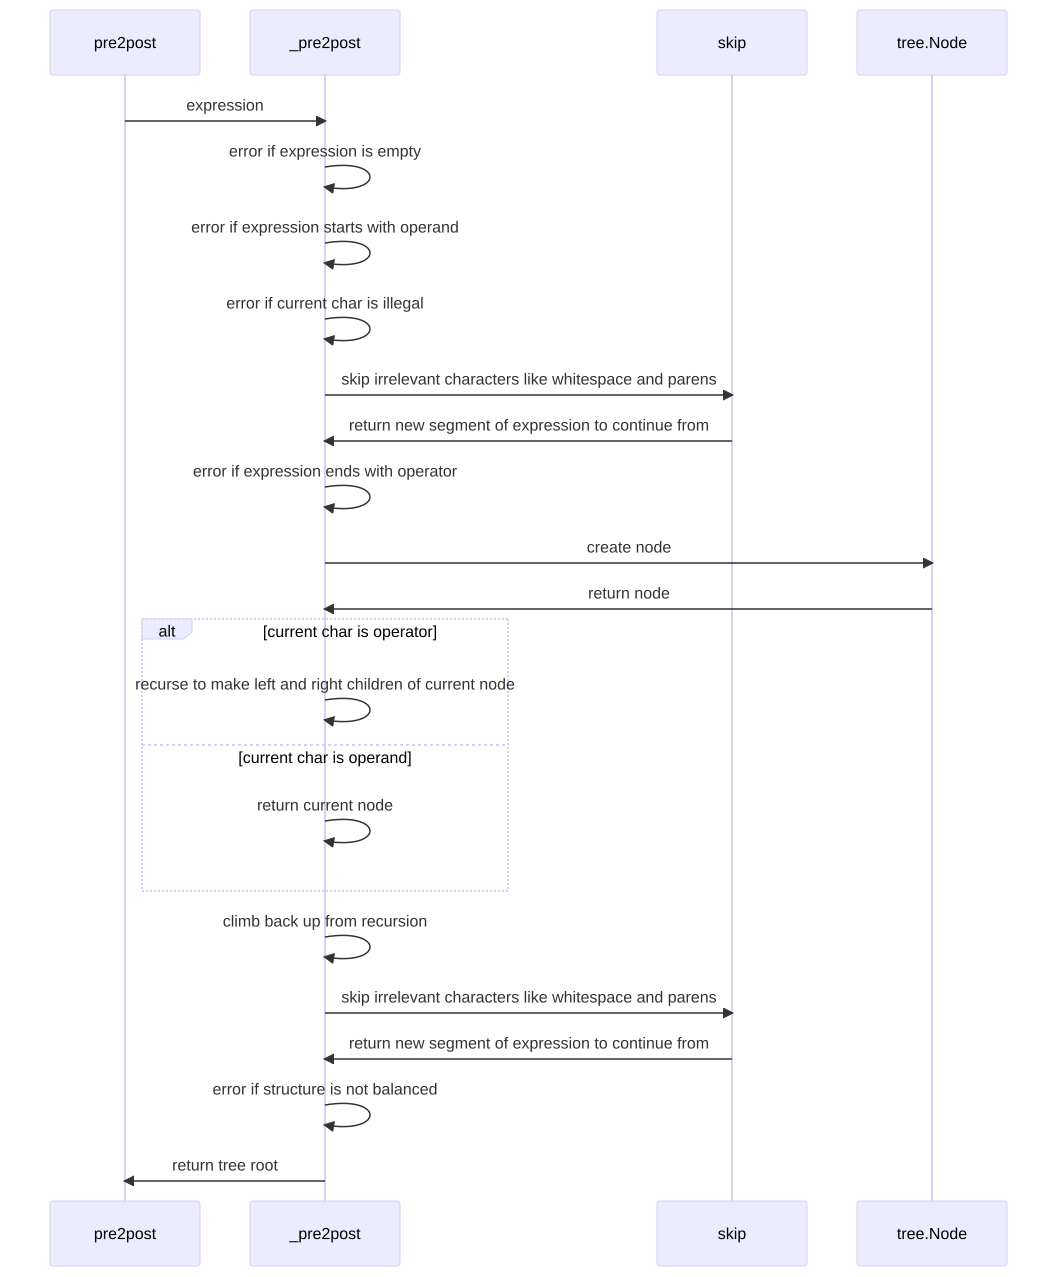
\includegraphics[width=0.9\linewidth]{lab2-strategy-validation.pdf}
  \caption{Validation flow}\label{fig:strategy-validation}
\end{figure}

\clearpage\pagebreak

\section{Structure}\label{sec:structure}

\begin{verbatim}
lab2
|-- __init__.py
|-- __main__.py
|-- convert
|   |-- __init__.py
|   |-- converter.py
|   `-- errors.py
|-- internal
|   |-- parse
|   |   |-- __init__.py
|   |   |-- cleaner.py
|   |   `-- validate.py
|   `-- tree
|       |-- __init__.py
|       `-- tree.py
|-- lab2.py
|-- launch.json
`-- tests
    |-- __init__.py
    |-- test_clean.py
    |-- test_converter.py
    `-- test_validate.py

6 directories, 16 files
\end{verbatim}

\section{Design Decisions}

Python lists are dynamic arrays of pointers to data objects \cite{PythonDocumentationDesignAndHistory}. The actual data items are stored separately, but indexing a list \texttt{a[i]} can be performed in $O(1)$, rather than needing to iterate through all the elements like in a linked list. These characteristics gave me some benefits for implementation. For example, because the array contains pointers, rather than the objects themselves, I was able to write my \texttt{Stack} class (see \autoref{sec:lab1/stack/stack.py}) to accept either data of type \texttt{str} or \texttt{int}, which meant that my functions for evaluating expressions (see \autoref{sec:strategy}) more straightforward to implement because they could just use the same stack used elsewhere.

Python's use of dynamic arrays instead of linked lists comes with another benefit, namely that the underlying layout of the pointers in memory is contiguous. The contiguity of the data makes it more likely that the data can be stored together in cache. Based on the locality principle used by many systems when retrieving information from resources like main memory or disc, if the data is contiguous in memory, then it is more likely that when a particular item is fetched from memory so too will the other items that are going to be needed in the near future. See Chapter 6 of \textcite{null2023essentials}, where there is a discussion of locality in memory management.

The performance of the stack's operations in my implementation are as follows:

\begin{center}
  \begin{tabularx}{\textwidth}{|l|l|X|}
    \hline
    Function                                      & Worst Case                 & Description                                                                                               \\ \hline
    \texttt{__init__(self, max_height: int = -1)} & $O(1)$                     & Only has to initialize an instance of Stack. Time complexity has no dependence on n or max_height.        \\ \hline
    \texttt{is_empty(self) -> bool}               & $O(1)$                     & Only has to read an attribute from the instance of Stack. Time complexity has no dependence on height.    \\ \hline
    \texttt{is_full(self) -> bool}                & $O(1)$                     & Only has to read an attribute from the instance of Stack. Time complexity has no dependence on height.    \\ \hline
    \texttt{contains(self, item) -> bool}         & $O(n)$                     & Has to iterate over each of the elements in the instance of Stack. In the worse case all must be checked. \\ \hline
    \texttt{peek(self) -> str | int | None}       & $O(1)$                     & Only has to check one element. Time complexity has no dependence on height.                               \\ \hline
    \texttt{pop(self) -> str | int | None}        & $O(1)$                     & Only has to return one element. Time complexity has no dependence on height.                              \\ \hline
    \texttt{push(self, item: str | int) -> None}  & $O(n)$ or $O(1)$ amortized & See note below.                                                                                           \\ \hline
  \end{tabularx}
\end{center}

Note on \texttt{push}: Because the Python list that contains the data is implemented as a dynamic array, when its capacity is filled, this will result in a resizing operation that takes $O(n)$ time. However, when looking at the average performance of \texttt{push}, the additional cost of the resizing operations reduces to a constant cost on average. This is because the frequency with which the resizing operations must be performed decreases exponentially as the size of the underlying array grows, under the assumption that the size of the array is doubled each time it is resized. See \textcite{EnWikipediaorgAmortizedAnalysis}, which will point to \textcite{Kozen2011CornellLectureAmortizedAnalysis}, which is itself a clarifying reformulation of \textcite{Tarjan1985AmortizedComputationalComplexity} for more details.


The following is the implementation of \texttt{converter.pre2post}, with the docstring and other long comments stripped out to save space. The full version is in \autoref{sec:lab1/convert/converter.py}. I have added notations for each step to indicate the time complexity required for the operation.


\begin{minted}[linenos,breaklines,breakanywhere=true,fontsize={\fontsize{7pt}{8pt}\selectfont}]{python}
def pre2post(expression: str) -> str:
    if not validate.is_valid_expression(expression=expression, expression_type="prefix"): # O(n)
        raise ValueError(f"'{expression}' is not a valid prefix expression")              # O(1)
    stack = Stack()                                                                       # O(1)
    parsed_expression = parser.parse(expression=expression)                               # O(n)
    postfix_expression_components = []                                                    # O(1)
    if parsed_expression == [] or len(parsed_expression) == 1:                            # O(1)
        return expression                                                                 # O(1)
    for i in range(0, len(parsed_expression)):  # iterate from right                      # O(n)
        index = len(parsed_expression) - (i + 1)                                          # O(1)
        symbol = parsed_expression[index]                                                 # O(1)
        if validate.is_parenthesis(symbol):                                               # O(1)
            continue                                                                      # O(1)
        if validate.is_operator(str(symbol)):                                             # O(1)
            a = stack.pop()                                                               # O(1)
            b = stack.pop()                                                               # O(1)
            stack.push(f"{a}{b}{symbol}")                                                 # O(1)
        elif isinstance(symbol, str):                                                     # O(1)
            stack.push(symbol)                                                            # O(1)
    while not stack.is_empty():                                                           # O(1)
        symbol = stack.pop()                                                              # O(n)/amortized O(1)
        postfix_expression_components.append(symbol)                                      # O(n)/amortized O(1)
    postfix_expression = "".join(postfix_expression_components)                           # O(n)
    return postfix_expression                                                             # O(1)
\end{minted}

The core of the preceding analysis applies similarly to the function \texttt{validate.is_valid_expression} (in \autoref{sec:lab1/parse/validate.py}) and to \texttt{parser.parse} (in \autoref{sec:lab1/parse/parser.py}).

From this, we can conclude that for each of the steps in the conversion pipeline, there are at most $kn$ steps, where $k \in \mathbb{Z^+}$ and $n$ is the length of the original expression. The time complexity's being an integer multiple of the size of the input implies that the worst case complexity is $O(n)$ for the program.


\section{Algorithms and ADTs}

For this lab, a stack is a reasonable ADT to use because of the structure of the problem itself. Prefix and postfix notation for mathematical expressions themselves are designed around stacks. As you read a symbol in either format, the determination of how to handle it is unambiguous because of the stack semantics inherent in the notation. This is in notable contrast to infix notation, with which there is ambiguity about evaluation order that must be disambiguated using parentheses.

Because the problem of parsing these expressions lends itself inherently a stack, it lends itself also naturally to a recursive implementation. A recursive implementation implicitly uses the stacks, and when evaluated, it will take advantage of the stack provided by the operating system to execute. The problem also semantically suggests a recursive definition, because it can be expressed using a context free grammar.

\begin{align*}
   & R \to XAA \mid RR                                                                 \\
   & X \to \texttt{+} \mid \texttt{-} \mid \texttt{*} \mid \texttt{/} \mid \texttt{\$} \\
   & A \to R\ | \texttt{Int}
\end{align*}

This reads that a variable $R$ can be replaced either by $XAA$ or a sequence of two variables $RR$. $X$ can be replaced by one of the terminal operators, and $A$ can be replaced either by another variable R or an integer. With this pattern, we can produce any prefix operation. The grammar for a postfix expression is the following:

\begin{align*}
   & R \to AAX \mid RR                                                                 \\
   & X \to \texttt{+} \mid \texttt{-} \mid \texttt{*} \mid \texttt{/} \mid \texttt{\$} \\
   & A \to R\ | \texttt{Int}
\end{align*}

Why does it matter that this can be expressed as a context free grammar (CFG)? Every CFG is computationally equivalent to a pushdown automaton (PDA) \cite{sipser2013}, which is a model of computation that only has states and a single stack that it can push and pop from. Context free grammars make clear that there is a recursive definition for any of the languages (i.e. computational problems) that they model. A recursive definition of the conversion problem would be more straightforward to implement and to reason about, because we would not have to manage the stack manipulation ourselves. This does not necessarily make the recursive definition of the problem better, since for a given language and for a given problem, a naive recursive solution to a problem may not make effective use of space, as we have seen in the case of calculating Fibonacci numbers recursively. However, the benefits of declarative, high-level functional programming are significant. Recursive functions lend themselves to such contexts, and given that there are compiler optimizations, intelligent memoization, and tail recursion available for us to use, I would recommend the use of a recursive solution to this and similar problems where possible. The manual state management of the stack is similar to memory management in system-level languages. There is usually a reasonable abstraction provided by an implemntation that handles the low-level details correctly, and using that abstraction is likely to reduce the likelihood of bugs and cognitive effort's being spent on implementation details when it could be spent modeling the domain appropriately. We don't need to reinvent sequence iteration every time we want to handle all the elements in a list. Instead, we could just use map and a function.

\pagebreak

\section{Testing}\label{sec:testing}

I predominantly used test-driven development with unit tests written in \texttt{unittest} to help with the development of my code and to ensure that I did not break portions of the codebase as I built new features, performed refactors, and did other chores. This was especially useful in this lab, because I was able to inherit the testing work I had done in lab1 to guide both the rewriting and the excising of unused code that I had written previously but no longer needed. One of the challenging aspects of the situation that I learned from was that in addition to needing to change the implementation details, I also needed to change some of the contracts to the behavior. This meant that several of the tests needed to be updated along the way to accomodate the refined understanding of the problem specification. Keeping the changes in implementation separate from changes in specification was challenging at times.

In my analysis for lab1, I said,
\begin{quote}
  My test writing strategy is drawn from sources like \citetitle{JamesLearnGoWithTests}, where I learned to write tests to specify an API contract for a package, set of functions, or entire program before implementing the features themselves. As I added features to this lab, I wrote the tests first, mocking out the functions that I would call, and then I implemented the features. Before and after each code change, I ran the full test suite, so that I could immediately detect and address any changes to the code that resulted in changes in behavior of the program that either satisfied or broke the constraints of the specification encoded in the tests. There are a few small functions that I extracted later on in the lab that are not as comprehensively covered by the tests. Consequently, there is not 100\% coverage for the codebase. I don't think this is necessarily needed. Rather, the goal that I aimed for was external contract coverage and guarantees across the packages and for the program as a whole, leaving details of the implementation of those specifications out of test. This is analogous to the behavior seen in writing tests for languages like Java and Go, which have conventions about private vs public methods or unexported vs exported functions, respectively.
\end{quote}
  
As in lab1, where possible, I followed the strategy of writing tests first. I used an experiments script to explore the interactions of the Node class and the recursive algorithm however, which meant that I wrote some of the tests around the recursive algorithm later. Complicating this practice further was that I also needed to rip out several portions of the validate tooling, since those were both relying on iterative implementations with a stack and were enforcing stricter versions of the problem specification than were appropriate. As a result, I was not as cleanly disciplined about the TDD cycle in this lab as I was in the development of lab1. In the future, I would explore ways of organizing my work to help me adhere more closely to that cycle, since I found that when I was more disciplined about sticking to it, the work actually was easier. This lab was more difficult, I suspect, because of that relaxation of the workflow.

That said, I still relied heavily on the tests, and I derived a lot of benefit from them. For instance, when I worked on excising sections of the codebase that were fairly central to lab1, I was able to proceed with confidence and assurance that the behavior was still correct, because I ran my entire test suite after each action, deletion, or refactor.


\noindent The idealized workflow for adding features is:

\begin{enumerate}
  \item Write a test that reflects an atomic aspect of the expected behavior.
  \item Validate that the test fails without the implementation in place.
  \item Write a minimal implementation that makes the test pass.
  \item Iterate with new tests.
\end{enumerate}

\noindent The complementary idealized workflow for making changes, including deletions is:

\begin{enumerate}
  \item Run all the tests and validate they all pass.
  \item Make a targeted change.
  \item Re-run all the tests and validate they all pass.
  \item If a test fails, fix the issue while preserving the desired change.
  \item Iterate.
\end{enumerate}

\noindent The third kind of workflow, for changing specifications, is:

\begin{enumerate}
  \item Run all the tests and validate they all pass.
  \item Make a targeted change to the specification.
  \item Re-run all the tests.
  \item If a test fails, fix the issue while preserving the desired change to the specification.
  \item Iterate.
\end{enumerate}

To run the tests, I used the built-in \texttt{unittest} module's \texttt{discover} command. As I proceeded, I ran tests by calling the following from \texttt{jhu-en-605-202-su26-data-structures/test-1}: \texttt{python -m unittest discover -s lab1/tests}. This printed test results like the following:

{\small
  \begin{verbatim}
python -m unittest discover -s lab2/tests                                     
.......................
----------------------------------------------------------------------
Ran 23 tests in 0.001s

OK
\end{verbatim}
}

\pagebreak
\section{Demo}\label{sec:demo}

For the following, I assume that I start in the root of the Github repository. From some appropriate location on your filesystem, clone the repository and move into the root of the repo.
  {\small
    \begin{verbatim}
  git clone https://github.com/jllovet/jhu-en-605-202-su26-data-structures.git
  cd jhu-en-605-202-su26-data-structures
\end{verbatim}
  }

\noindent From there, move into the folder for this lab.

  {\small
    \begin{verbatim}
  cd lab-2
\end{verbatim}
  }

\noindent From here, the python module can be run as follows.

  {\small
    \begin{verbatim}
  python3 -m lab2 resources/input/in.txt resources/output/output.txt
\end{verbatim}
  }

\noindent If the program is run with the incorrect number of arguments, then an error message similar to the one shown below will be printed to the user.

\begin{minted}[breaklines, breakanywhere, fontsize=\footnotesize]{text}
python -m lab1
usage: python3.14 -m lab2 [-h] [-l {INFO,WARNING,ERROR,DEBUG,CRITICAL,FATAL}] [-f LOGFILE] in_file out_file

Convert prefix -> postfix expressions from in_file and write them to out_file

positional arguments:
  in_file               Input File Pathname
  out_file              Output File Pathname

options:
  -h, --help            show this help message and exit
  -l, --level {INFO,WARNING,ERROR,DEBUG,CRITICAL,FATAL}
                        Sets the level of the logger. Default INFO
  -f, --logfile LOGFILE
                        Sets the filename where logs are written
\end{minted}

\noindent The input and resulting output of an example successful run are shown below:

\begin{center}
  \begin{minipage}[t]{0.2\textwidth}
    \centering
    \textbf{\texttt{resources/input/in.txt}}\\
    \inputminted[frame=single,fontsize=\footnotesize]{text}{resources/input/in.txt}
  \end{minipage}\hfill
  \begin{minipage}[t]{0.76\textwidth}
    \centering
    \textbf{\texttt{resources/output/output.txt}}\\
    \inputminted[breaklines, breakanywhere, fontsize=\footnotesize, frame=single, fontsize=\footnotesize]{text}{resources/output/output.txt}
  \end{minipage}
\end{center}

\noindent When the program is executed as below, the message on the following page will be written to \texttt{stderr}:

\pagebreak

\begin{minted}[breaklines, breakanywhere, fontsize=\footnotesize]{text}
python -m lab2 resources/input/in.txt resources/output/output.txt    
Processing expressions below:
-+ABC
-A+BC
$+-ABC+D-EF
-*A$B+C-DE*EF
**A+BC+C-BA
/A+BC +C*BA  
*-*-ABC+BA  
/+/A-BC-BA  
*$A+BC+C-BA 
//A+B0-C+BA
*$A^BC+C-BA

WARNING: 5 errors found during conversion!
Check expressions are well-formed prefix expressions and only use allowed symbols.

Allowed symbols are alphabetical characters and any of: +-*/$()

Example valid expressions:
(base case):    'A'     -> 'A'
(single op):    '+AB'   -> 'AB+'
(more ops):     '-+ABC' -> 'AB+C-'
--------------------------------------------------------------------------------
ERROR: resources/input/in.txt - line 6: '/A+BC +C*BA  ' could not be processed. Please ensure it has a valid prefix structure.
ERROR: resources/input/in.txt - line 7: '*-*-ABC+BA  ' has too many operators.
ERROR: resources/input/in.txt - line 8: '/+/A-BC-BA  ' has too many operators.
ERROR: resources/input/in.txt - line 10: '//A+B0-C+BA' has an illegal character '0' at position 6.
ERROR: resources/input/in.txt - line 11: '*$A^BC+C-BA                                   ' has an illegal character '^' at position 4.
\end{minted}

\pagebreak
\section{Enhancements and What I Learned}\label{sec:enhancements-and-what-I-learned}

\noindent \textbf{Enhancement: Unit Testing - Validations on Single Passes}
\medskip

For details of the unit testing that I did as an enhancement, please see \ref{sec:testing}.

Building in validations of correctness without additional passes was significantly more difficult than I had anticipated. It's much easier to ensure correctness when multiple passes are allowed, since in those cases you can answer questions about the structure of the whole of the input. With the constraint of performing a single pass over the input, the problem of solution verification must rely on characteristics that can be determined by partial information, which sometimes is insufficient. In the future, I will try to model this more effectively to have a cleaner implementation, especially in the case that I am writing a recursive function, where the mental overhead is slightly higher than in iterative solutions.

\medskip
\noindent \textbf{Enhancement: Logging}
\medskip

This version of the lab uses the python logging package to write logs. Most of these are configured to only be emitted when the logger leve is set to debug, but there are a number of logs that are produced at an info and error level. The log level can be set by the user through the command line. By default this is Recall the usage:

\begin{minted}[breaklines, breakanywhere, fontsize=\footnotesize]{text}
usage: python3 -m lab2 [-h] [-l {INFO,WARNING,ERROR,DEBUG,CRITICAL,FATAL}]
                          [-f LOGFILE]
                          in_file out_file

Convert prefix -> postfix expressions from in_file and write them to out_file

positional arguments:
  in_file               Input File Pathname
  out_file              Output File Pathname

options:
  -h, --help            show this help message and exit
  -l, --level {INFO,WARNING,ERROR,DEBUG,CRITICAL,FATAL}
                        Sets the level of the logger. Default INFO
  -f, --logfile LOGFILE
                        Sets the filename where logs are written
\end{minted}

To set the log level to DEBUG, for example, the user could run a command like the following:

\begin{minted}[breaklines, breakanywhere, fontsize=\footnotesize]{text}
python -m lab2 resources/input/readme.txt resources/output/output.txt --level DEBUG
\end{minted}

Similarly, the user can set the name of the logfile. 

\begin{minted}[breaklines, breakanywhere, fontsize=\footnotesize]{text}
python -m lab2 resources/input/readme.txt resources/output/output.txt --level DEBUG --logfile mylab2.log
\end{minted}

This will produce a logfile called \texttt{mylab2.log} with the contents below:

\begin{minted}[breaklines, breakanywhere, fontsize=\footnotesize]{text}
2026-07-15T01:21:01-0400 - [__main__.py:<module>:46] - INFO - processing input file resources/input/readme.txt and writing to resources/output/output.txt
2026-07-15T01:21:01-0400 - [lab2.py:process_files:41] - INFO - Beginning to process expressions
2026-07-15T01:21:01-0400 - [converter.py:pre2post:307] - INFO - Attempting to convert: 'A'
2026-07-15T01:21:01-0400 - [converter.py:_pre2post:134] - DEBUG - Considering whether to skip characters
2026-07-15T01:21:01-0400 - [converter.py:_pre2post:135] - DEBUG - CURRENT: 'A'
2026-07-15T01:21:01-0400 - [converter.py:_pre2post:152] - DEBUG - MAKING NODE FROM:'A'
2026-07-15T01:21:01-0400 - [converter.py:pre2post:314] - DEBUG - POSTFIX EXPRESSION: 'A'
2026-07-15T01:21:01-0400 - [lab2.py:process_files:46] - DEBUG - Converted 'A' -> 'A'
2026-07-15T01:21:01-0400 - [converter.py:pre2post:307] - INFO - Attempting to convert: 'AB'
2026-07-15T01:21:01-0400 - [converter.py:_pre2post:120] - ERROR - 'AB' could not be processed. Prefix expressions can't start with an operand.
2026-07-15T01:21:01-0400 - [converter.py:pre2post:317] - ERROR - Reraising error: 'AB' could not be processed. Prefix expressions can't start with an operand.
2026-07-15T01:21:01-0400 - [converter.py:pre2post:307] - INFO - Attempting to convert: 'AB+'
2026-07-15T01:21:01-0400 - [converter.py:_pre2post:120] - ERROR - 'AB+' could not be processed. Prefix expressions can't start with an operand.
2026-07-15T01:21:01-0400 - [converter.py:pre2post:317] - ERROR - Reraising error: 'AB+' could not be processed. Prefix expressions can't start with an operand.
2026-07-15T01:21:01-0400 - [converter.py:pre2post:307] - INFO - Attempting to convert: '+AA'
2026-07-15T01:21:01-0400 - [converter.py:_pre2post:134] - DEBUG - Considering whether to skip characters
2026-07-15T01:21:01-0400 - [converter.py:_pre2post:135] - DEBUG - CURRENT: '+'
2026-07-15T01:21:01-0400 - [converter.py:_pre2post:161] - DEBUG - CURRENT CHAR:+
2026-07-15T01:21:01-0400 - [converter.py:_pre2post:162] - DEBUG - MAKING NODE FROM:'+'
2026-07-15T01:21:01-0400 - [converter.py:_pre2post:167] - DEBUG - FOUND OPERATOR:+
2026-07-15T01:21:01-0400 - [converter.py:_pre2post:134] - DEBUG - Considering whether to skip characters
2026-07-15T01:21:01-0400 - [converter.py:_pre2post:135] - DEBUG - CURRENT: 'A'
2026-07-15T01:21:01-0400 - [converter.py:_pre2post:161] - DEBUG - CURRENT CHAR:A
2026-07-15T01:21:01-0400 - [converter.py:_pre2post:162] - DEBUG - MAKING NODE FROM:'A'
2026-07-15T01:21:01-0400 - [converter.py:_pre2post:134] - DEBUG - Considering whether to skip characters
2026-07-15T01:21:01-0400 - [converter.py:_pre2post:135] - DEBUG - CURRENT: 'A'
2026-07-15T01:21:01-0400 - [converter.py:_pre2post:152] - DEBUG - MAKING NODE FROM:'A'
2026-07-15T01:21:01-0400 - [converter.py:_pre2post:214] - DEBUG - AT DEPTH 0: OPERATORS:1 OPERANDS:2
2026-07-15T01:21:01-0400 - [converter.py:pre2post:314] - DEBUG - POSTFIX EXPRESSION: 'AA+'
2026-07-15T01:21:01-0400 - [lab2.py:process_files:46] - DEBUG - Converted '+AA' -> 'AA+'
2026-07-15T01:21:01-0400 - [lab2.py:process_files:65] - WARNING - Errors raised
2026-07-15T01:21:01-0400 - [converter.py:pre2post:307] - INFO - Attempting to convert: 'A'
2026-07-15T01:21:01-0400 - [converter.py:_pre2post:134] - DEBUG - Considering whether to skip characters
2026-07-15T01:21:01-0400 - [converter.py:_pre2post:135] - DEBUG - CURRENT: 'A'
2026-07-15T01:21:01-0400 - [converter.py:_pre2post:152] - DEBUG - MAKING NODE FROM:'A'
2026-07-15T01:21:01-0400 - [converter.py:pre2post:314] - DEBUG - POSTFIX EXPRESSION: 'A'
2026-07-15T01:21:01-0400 - [converter.py:pre2post:307] - INFO - Attempting to convert: '+AB'
2026-07-15T01:21:01-0400 - [converter.py:_pre2post:134] - DEBUG - Considering whether to skip characters
2026-07-15T01:21:01-0400 - [converter.py:_pre2post:135] - DEBUG - CURRENT: '+'
2026-07-15T01:21:01-0400 - [converter.py:_pre2post:161] - DEBUG - CURRENT CHAR:+
2026-07-15T01:21:01-0400 - [converter.py:_pre2post:162] - DEBUG - MAKING NODE FROM:'+'
2026-07-15T01:21:01-0400 - [converter.py:_pre2post:167] - DEBUG - FOUND OPERATOR:+
2026-07-15T01:21:01-0400 - [converter.py:_pre2post:134] - DEBUG - Considering whether to skip characters
2026-07-15T01:21:01-0400 - [converter.py:_pre2post:135] - DEBUG - CURRENT: 'A'
2026-07-15T01:21:01-0400 - [converter.py:_pre2post:161] - DEBUG - CURRENT CHAR:A
2026-07-15T01:21:01-0400 - [converter.py:_pre2post:162] - DEBUG - MAKING NODE FROM:'A'
2026-07-15T01:21:01-0400 - [converter.py:_pre2post:134] - DEBUG - Considering whether to skip characters
2026-07-15T01:21:01-0400 - [converter.py:_pre2post:135] - DEBUG - CURRENT: 'B'
2026-07-15T01:21:01-0400 - [converter.py:_pre2post:152] - DEBUG - MAKING NODE FROM:'B'
2026-07-15T01:21:01-0400 - [converter.py:_pre2post:214] - DEBUG - AT DEPTH 0: OPERATORS:1 OPERANDS:2
2026-07-15T01:21:01-0400 - [converter.py:pre2post:314] - DEBUG - POSTFIX EXPRESSION: 'AB+'
2026-07-15T01:21:01-0400 - [converter.py:pre2post:307] - INFO - Attempting to convert: '-+ABC'
2026-07-15T01:21:01-0400 - [converter.py:_pre2post:134] - DEBUG - Considering whether to skip characters
2026-07-15T01:21:01-0400 - [converter.py:_pre2post:135] - DEBUG - CURRENT: '-'
2026-07-15T01:21:01-0400 - [converter.py:_pre2post:161] - DEBUG - CURRENT CHAR:-
2026-07-15T01:21:01-0400 - [converter.py:_pre2post:162] - DEBUG - MAKING NODE FROM:'-'
2026-07-15T01:21:01-0400 - [converter.py:_pre2post:167] - DEBUG - FOUND OPERATOR:-
2026-07-15T01:21:01-0400 - [converter.py:_pre2post:134] - DEBUG - Considering whether to skip characters
2026-07-15T01:21:01-0400 - [converter.py:_pre2post:135] - DEBUG - CURRENT: '+'
2026-07-15T01:21:01-0400 - [converter.py:_pre2post:161] - DEBUG - CURRENT CHAR:+
2026-07-15T01:21:01-0400 - [converter.py:_pre2post:162] - DEBUG - MAKING NODE FROM:'+'
2026-07-15T01:21:01-0400 - [converter.py:_pre2post:167] - DEBUG - FOUND OPERATOR:+
2026-07-15T01:21:01-0400 - [converter.py:_pre2post:134] - DEBUG - Considering whether to skip characters
2026-07-15T01:21:01-0400 - [converter.py:_pre2post:135] - DEBUG - CURRENT: 'A'
2026-07-15T01:21:01-0400 - [converter.py:_pre2post:161] - DEBUG - CURRENT CHAR:A
2026-07-15T01:21:01-0400 - [converter.py:_pre2post:162] - DEBUG - MAKING NODE FROM:'A'
2026-07-15T01:21:01-0400 - [converter.py:_pre2post:134] - DEBUG - Considering whether to skip characters
2026-07-15T01:21:01-0400 - [converter.py:_pre2post:135] - DEBUG - CURRENT: 'B'
2026-07-15T01:21:01-0400 - [converter.py:_pre2post:161] - DEBUG - CURRENT CHAR:B
2026-07-15T01:21:01-0400 - [converter.py:_pre2post:162] - DEBUG - MAKING NODE FROM:'B'
2026-07-15T01:21:01-0400 - [converter.py:_pre2post:134] - DEBUG - Considering whether to skip characters
2026-07-15T01:21:01-0400 - [converter.py:_pre2post:135] - DEBUG - CURRENT: 'C'
2026-07-15T01:21:01-0400 - [converter.py:_pre2post:152] - DEBUG - MAKING NODE FROM:'C'
2026-07-15T01:21:01-0400 - [converter.py:_pre2post:214] - DEBUG - AT DEPTH 0: OPERATORS:2 OPERANDS:3
2026-07-15T01:21:01-0400 - [converter.py:pre2post:314] - DEBUG - POSTFIX EXPRESSION: 'AB+C-'
2026-07-15T01:21:01-0400 - [lab2.py:print_errors:105] - ERROR - ERROR: resources/input/readme.txt - line 2: 'AB' could not be processed. Prefix expressions can't start with an operand.
2026-07-15T01:21:01-0400 - [lab2.py:print_errors:105] - ERROR - ERROR: resources/input/readme.txt - line 3: 'AB+' could not be processed. Prefix expressions can't start with an operand.
\end{minted}

Inspection of the log file produced reveals that the log messages have a timestamp, the file, function, and line number where the log was produced, along with the severity of the message. (Note that the repetition of "ERROR" is because the second instance is shown to the user. It's part of the actual error message in this case.)

\noindent Some considerations:

By working through the implementation, I learned about the configuration of loggers in python, including how to set the log level and specify log outputs through calculated or user-provided values, such as I did in \texttt{lab2/__main__.py}. A similar approach could be used to mnaipulate the logger dynamically using environment variables or perhaps system capacity that was dynamically calculated (for instance, if the log volume written to disk was growing at a certain rate, the log level could be adjusted to accommodate).

I also found that there is a nuanced balance to find between abstraction, collocation, and code readability. What do I mean? While working on the logging I perform while raising errors, I found that the code was becoming more difficult to follow because of the proliferation of logging statements. To simplify the code, I considered that there would be a call to the logger whenever I raised a custom error. So, why not put the log into the error initialization directly, rather than write the log immediately before raising the error? This did in fact improve the main code readability, but it also resulted in losing the context of the issue when reading through the logs. Why? My logger here is configured to provide the file, the function, and the line number all together with the error message and timestamp. When I extracted the log write to the \texttt{__init__} function of the custom errors, I lost that rich context. Since the errors are really best used to investigate specific issues with an expression, it didn't make sense to make this tradeoff, and so I opted for a different refinement that left the logging calls in their original locations.

\medskip
\noindent \textbf{Enhancement: Testing on \texttt{isalpha()}}
\medskip

In the refinement of the specification that I discussed with the instructor, he suggested that I instead use \texttt{str.isalpha()} to determine whether a character is a valid operand. I discovered while writing tests for the new lab implementation that \texttt{str.isalpha()} returned \texttt{True} for symbols from other alphabets as well as the latin alphabet. This means that there can be quite amusing combinations of symbols that are used as operands in the expressions (though perhaps this is characteristic of real mathematical typesetting and shouldn't be surprising)! 

See the example below that shows that the converter succeeds even when mixing multiple alphabets, even if they are written in different directions. (The example uses polytonic Ancient Greek, Russian, and Hebrew letters.)

\begin{figure}[ht]
  \centering
  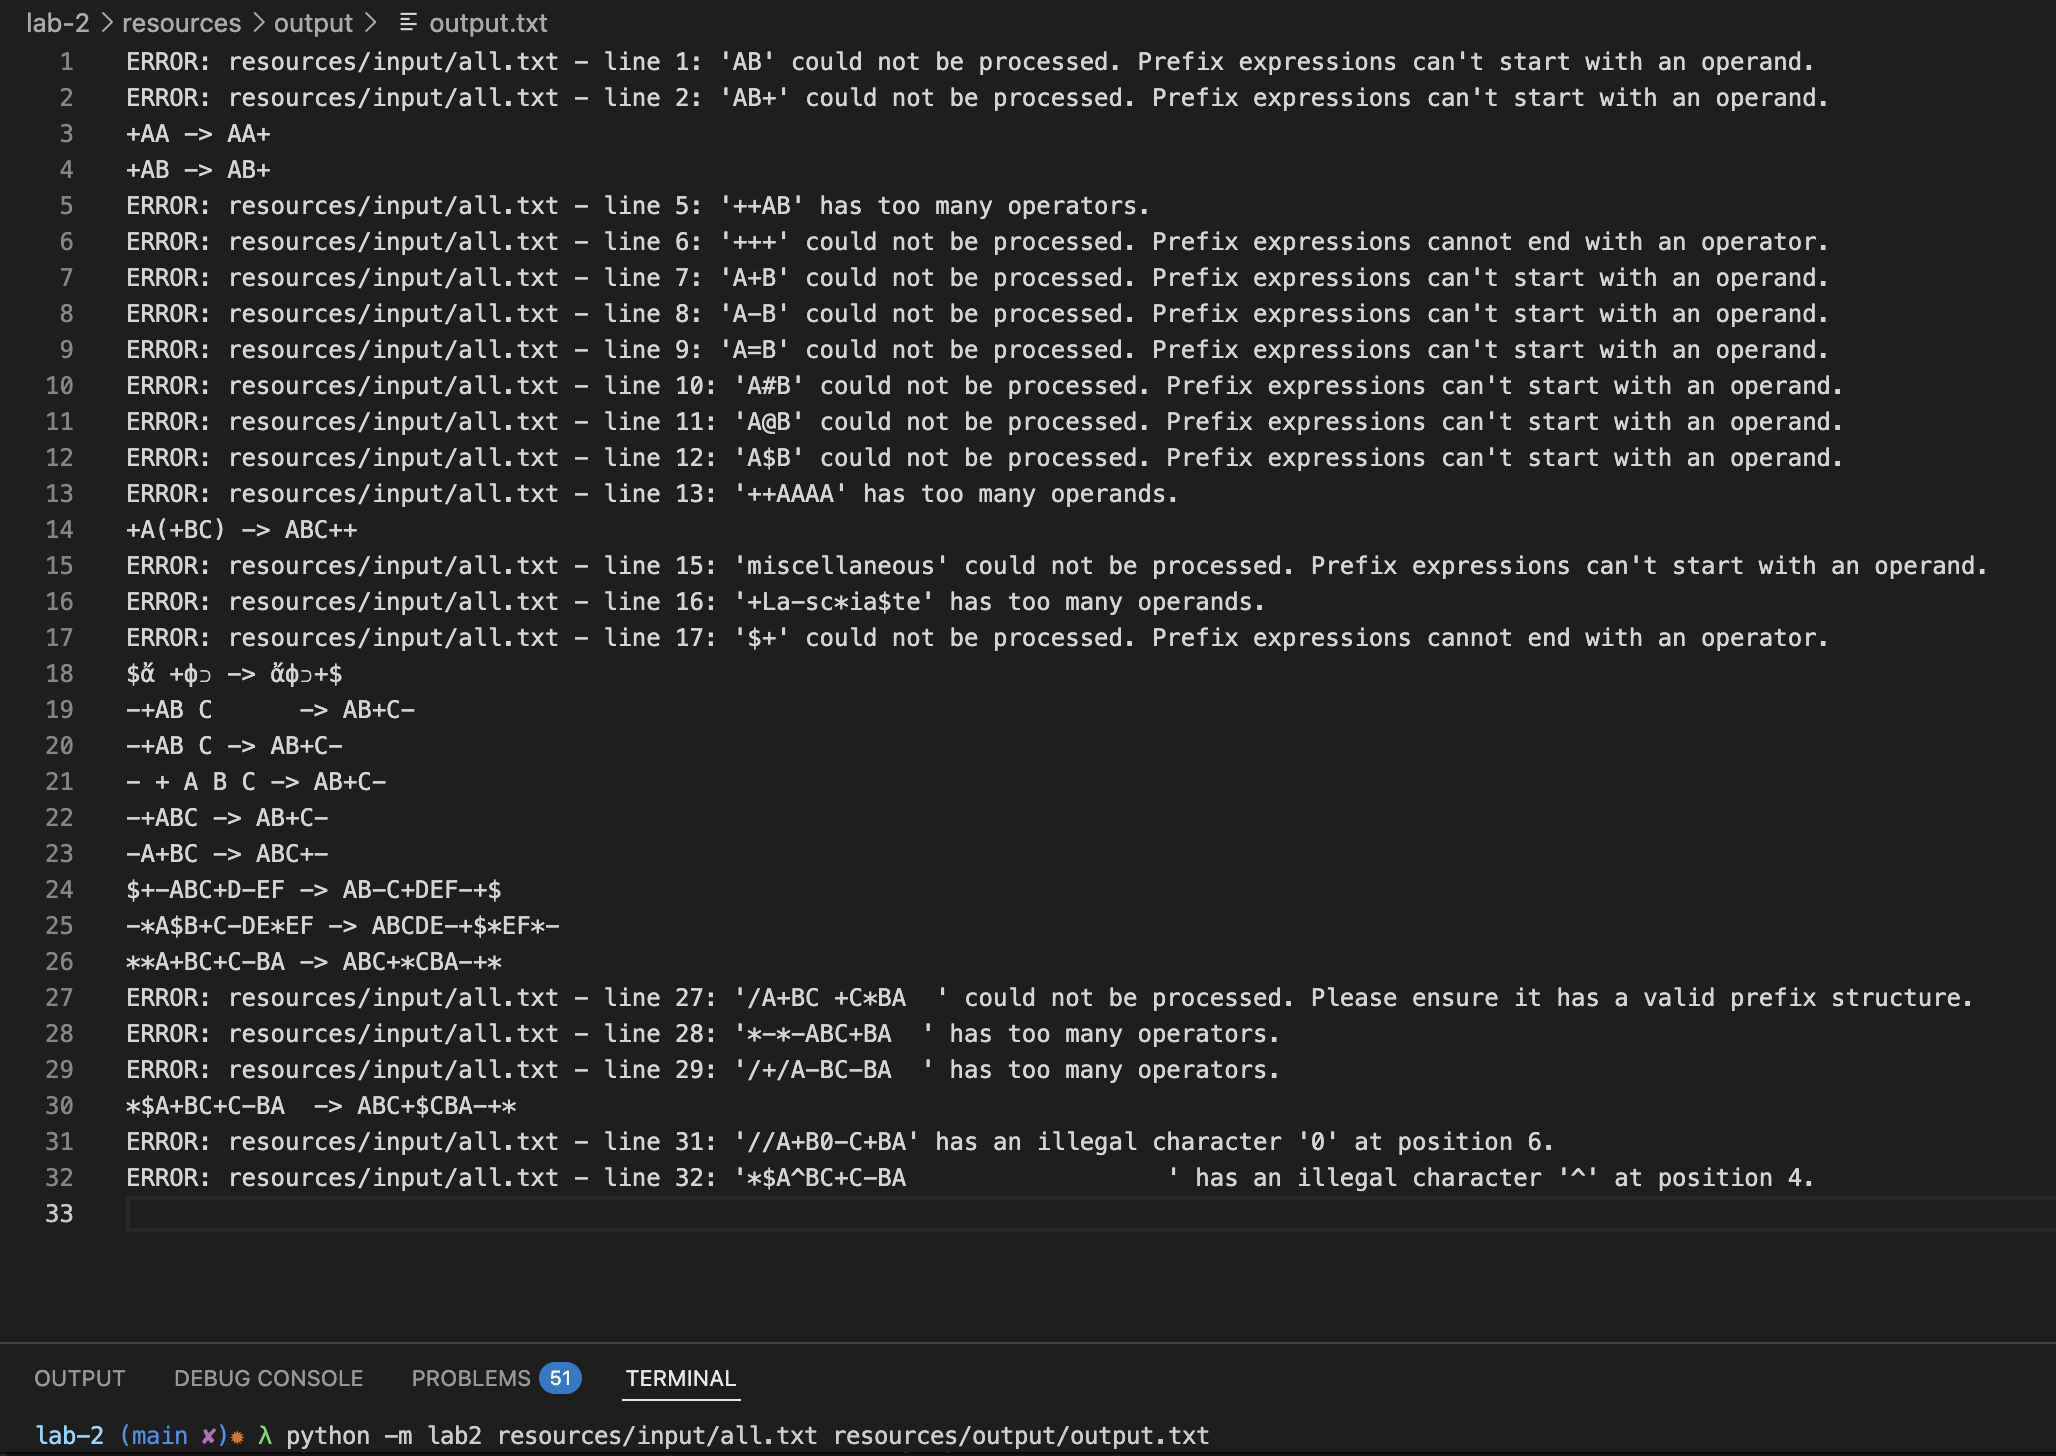
\includegraphics[width=0.9\linewidth]{screenshot-multialphabet-conversions.png}
  \caption{Screenshot of Multi-Alphabet Conversion on Line 18}\label{fig:multialphabet-conversions}
\end{figure}

\clearpage

\noindent \textbf{Generators and Yields}

Based on a conversation with the professor during office hours, I experimented in this lab with using python's generators. Using \texttt{yield} in the \texttt{__iter__} function of the \texttt{Node} class in the correct order, I was able to make extracting the postfix expression from the tree simple. I form an abstract syntax tree, and then I use the \texttt{__iter__} function to iterate over the nodes in post-order, meaning that I start with the leaves, reading the left child, then the right child, then the parent, left to right, up the tree recursively. In the future I will experiment more with using generators and iterators to have lazy evaluation in python.

While I read and watched multiple resources to learn about generators, I'm especially indebted to the strategy described here: \url{https://martinheinz.dev/blog/88}.

Here is \texttt{Node.__iter__}:

\begin{minted}[breaklines, breakanywhere, fontsize=\footnotesize]{python}
def __iter__(self):
    """Yield the nodes of the tree in post-order

    Inspired by the strategy described here: https://martinheinz.dev/blog/88
    
    Args:
        None

    Returns:
        Yields the elements of the tree in post-order.

    Raises:
        None

    Side Effects:
        None

    Idempotent:
        False
    """
    if self.left:
        yield from self.left
    if self.right:
        yield from self.right
    yield self.data
\end{minted}

\noindent \textbf{Custom Error Types}
In addition to the items above, I inlcuded custom error types in this lab, to experiment with the inheritance and the pattern of specific sentinel error types. They allow for more precise error types in the function \texttt{_pre2post} than \texttt{ValueError}, for example. The illustration below shows how I defined a base custom error class: \texttt{InvalidExpressionError}, which itself inherits from \texttt{ValueError}. From there there are three child error types inheriting from it, each with its own default error message.

\begin{minted}[breaklines, breakanywhere, fontsize=\footnotesize]{python}
class InvalidExpressionError(ValueError):
    def __init__(self, msg: str):
        super().__init__(msg)


class TooManyOperatorsError(InvalidExpressionError):
    def __init__(self, msg: str = "Too many operators provided in expression"):
        super().__init__(msg)


class TooManyOperandsError(InvalidExpressionError):
    def __init__(self, msg: str = "Too many operands provided in expression"):
        super().__init__(msg)


class IllegalOperandError(InvalidExpressionError):
    def __init__(self, msg: str = "Illegal operand provided in expression"):
        super().__init__(msg)
\end{minted}

This experiment was prompted also by discussion with our instructor. I am curious to see how more complex designs that use this pattern work, both at the project level and at the ecosystem level. For example, if you were a consumer of a package like this, you would need to handle the custom error types, meaning anywhere you have code that consumes anything that does not handle that for you, the errors package for this package becomes an import dependency. This could be handled by the package itself handling converting custom errors into standard library errors, but if that were done systematically, there would need to be quite a lot of benefit to make this additional engineering of error types worthwhile for consumers of the package.

\pagebreak

\section{Resouces Referenced While Coding}

In addition to the resources I mentioned above, I reviewed multiple resources for information about generators and iterators in python. In particular:

\begin{enumerate}
  \item \fullcite{PythondocumentationExpressions}
  \item \fullcite{StackOverflowDifferenceBetweenPythonsGeneratorsAndIterators}
  \item \fullcite{RedditcomCanSomeonePleaseExplainWhatIsAGenerator}
  \item \fullcite{PythonEnhancementProposalsPEP255}
  \item \fullcite{StackOverflowUnderstandingGeneratorsIn}
  \item \fullcite{RedditcomCanYouMakeAnInfiniteGeneratorWithGeneratorExpressionSyntax}
  \item \fullcite{PythondocumentationItertoolsFunctions}
  \item \fullcite{CoreySchafer2015PythonTutorialGenerators}
  \item \fullcite{MCoding2022PythonGenerators}
  \item \fullcite{ArjanCodes2026WhatMostPython}
  \item \fullcite{NeuralNine2021GeneratorsAdvanced}
\end{enumerate}

I am especially indebted to \textcite{Martinheinzdev2023LazyEvaluationUsing} for the idea on how to use \texttt{yield} to allow me to traverse the abstract syntax tree for my expression in post-order, effectively letting me read off the postfix expresssion directly from the tree.

A few other sources I referenced include \textcite{PythonDocumentationTypingLiterals} for information on Python typing, and the Google Python Style Guide \textcite{GooglePythonStyleGuide} as a basis for an internal standard for docstring formatting. I departed slightly from the Google convention, notably in adding sections of the docstring to describe functions' side effects and whether the function is idempotent.

\pagebreak

\section{Source Code}
The full source code, including LaTeX, tooling, other artifacts, and git history is available on my Github repository for the class here:
\begin{center}
  \url{https://github.com/jllovet/jhu-en-605-202-su26-data-structures}
\end{center}

\printbibliography[heading=bibintoc]

\end{document}